\section{Évaluation du projet}

Dans cette partie, nous allons faire une évaluation du projet. Nous évaluerons d'abord le logiciel dans ses trois principales parties. Ensuite, nous verrons son utilisabilité pour les artistes et l'écriture de la chorégraphie. Enfin, d'une manière plus générale, nous aborderons la gestion du projet. 

\subsection{Validation du logiciel} %validation des fonctionnalités du logiciel 

Dans cette partie, nous vérifions que les principales fonctionnalités sont correctes. On s'intéressera aux trois parties du logiciel séparément: la visualisation, la communication et la simulation. 

\subsubsection{Visualisation}

Concernant la visualisation, les trois critères importants pour évaluer cette partie sont : la fluidité des mouvements, la maniabilité de l'environnement 3D et l'ergonomie de l'interface utilisateur. 

La fluidité des images est assurée par un nombre d'images par seconde fixé à 60 fps, ce qui permet d'avoir un rendu agréable et fluide. La chorégraphie imaginée par les étudiants compterait 10 robots metabot, et dans ces conditions le nombre d'images par seconde est toujours 60 fps : l'image est fluide et l'interface réagit instantanément (pour un utilisateur, la différence de vitesse ne se sent pas entre 1 et 10 robots).
Nous avons testé pour 100 robots, le lancement de l'application prend du temps et le nombre d'images par seconde est divisé par 2, on a donc 30 fps ce qui reste correct pour une visualisation. 

La maniabilité de l'environnement 3D repose principalement sur les déplacements de la camera de type rotation et zoom. Les deux sont rendus possibles grâce à la classe \verb|EasyCam| d'openFrameworks qui permet d'avoir une camera simple munie des fonctionnalités usuelles (rotation, zoom, calibrage à l'initialisation automatique par rapport au milieu de la scène). Ainsi, l'utilisateur retrouve un environnement 3D usuel.

Nous avons essayé de penser à l'ergonomie, en rajoutant des menus déroulant pour chaque robot dans l'interface, ce qui permet d'éviter que le panel n'envahisse tout l'écran. De plus, un message d'aide est affiché au lancement du logiciel, il explique les touches à appuyer pour afficher des axes ou la graduation en plus, et aussi pour cacher ce message d'aide.
De même l'affichage de message de sélection permet à l'utilisateur d'identifier facilement les robots, sans qu'il ait à regarder le panel des positions.

Par ailleurs, pour alerter l'utilisateur de collision, nous avons choisi d'afficher un cercle rouge à l'emplacement du cercle mais aussi d'afficher un message informatif en haut de l'écran. Cela permet d'assurer que cet événement soit bien visible. En effet, si l'utilisateur zoom sur d'autres robots, il risque de ne pas voir le cercle rouge, alors que le message est toujours affiché au même endroit puisqu'il ne dépend pas de la scène 3D. Le cercle rouge permet tout comme le message de sélection, d'identifier plus facilement l'emplacement de la collision.

\subsubsection{Communication réseau}

Au niveau de la communication, nous avons comparé la fréquence d'appel à la méthode \verb|update| de la classe \verb|ofApp| de mise à jour de la scène par rapport à la fréquence d'i-score. En effet, on pourrait avoir des problèmes de temps si la méthode \verb|update| était appelée à une fréquence moins élevée que le tic d'i-score car on pourrait avoir des données d'i-score qui ne seraient pas mises à jour dans simulationRainOfmusic : par exemple si la fonction \verb|update| est appelée toutes les 50 ms et que le tic d'i-score est de 20 ms. 

En réalité, la méthode \verb|update| est appelée toute les 16 ms et le tic d'i-score est de 40 ms par défaut. Ainsi, les données utilisées par simulationRainOfMusic sont toujours synchronisées par rapport à celles d'i-score. On pourrait même imaginer une petite diminution de la fréquence d'appel à \verb|update| pour soulager l'utilisation de ressources, notamment lors d'une représentation avec beaucoup de robots. 

Par ailleurs, comme simulationRainOfMusic a un taux de rafraîchissement plus élevé, certaines données ne sont pas mises à jour dans i-score, notamment lorsque l'utilisateur modifie des paramètres à l'aide d'un slider via l'interface. Cependant le logiciel i-score possède la possibilité de faire des interpolations, ainsi il n'est pas nécessaire qu'i-score reçoive toutes les modifications au niveau de l'interface de simulationRainOfMusic. 

\subsubsection{Simulation}

A propos de la simulation du logiciel, plusieurs aspects peuvent être vérifiés.

D'abord, l'échelle spatio-temporelle : chaque graduation représente un mètre et si un metabot reçoit les commandes indiquant des mouvements de vitesse $dx=100 mm.s^{-1}$ ou $dy=100 mm.s^{-1}$, celui-ci avance bien d'une graduation toutes les dix secondes.

Ensuite, la consommation de la batterie des robots se fait bien linéairement en fonction de la distance parcourue par le robot en question. Si on fait parcourir dix mètres à un robot, une même quantité de batterie est consommée sur chaque mètre. A l'arrêt, les robots ne consomment pas. Des expérimentations pourraient être faites pour avoir un modèle de consommation plus réaliste. Par exemple, on pourrait s'intéresser à la consommation à l'arrêt ou selon la vitesse et la fréquence de pas quand le metabot est en mouvement.

Enfin, pour la perte de paquet, on peut compter le nombre de paquets perdus et reçus et retrouver le pourcentage de perte correspondant. Pour que celui-ci soit réaliste, on pourrait faire des expérimentations pour l'évaluer mais le protocole de communication n'est pas encore décidé définitivement (Bluetooth ou XBee). 

\subsection{Confrontation du logiciel avec les artistes}

Dans le cadre d'une rencontre avec les artistes, nous avons pu commencer à écrire la chorégraphie qu'ils avaient conçu. Ainsi les deux figures suivantes présentent un des tableaux que les artistes avaient conçu (figure \ref{chore}), et la visusalisation avec notre logiciel (figure \ref{reveil}). La chorégraphie dans son ensemble est en Annexe sous forme de storyboard. 


%\hspace*{-12cm}
\begin{figure}[H]
\centering
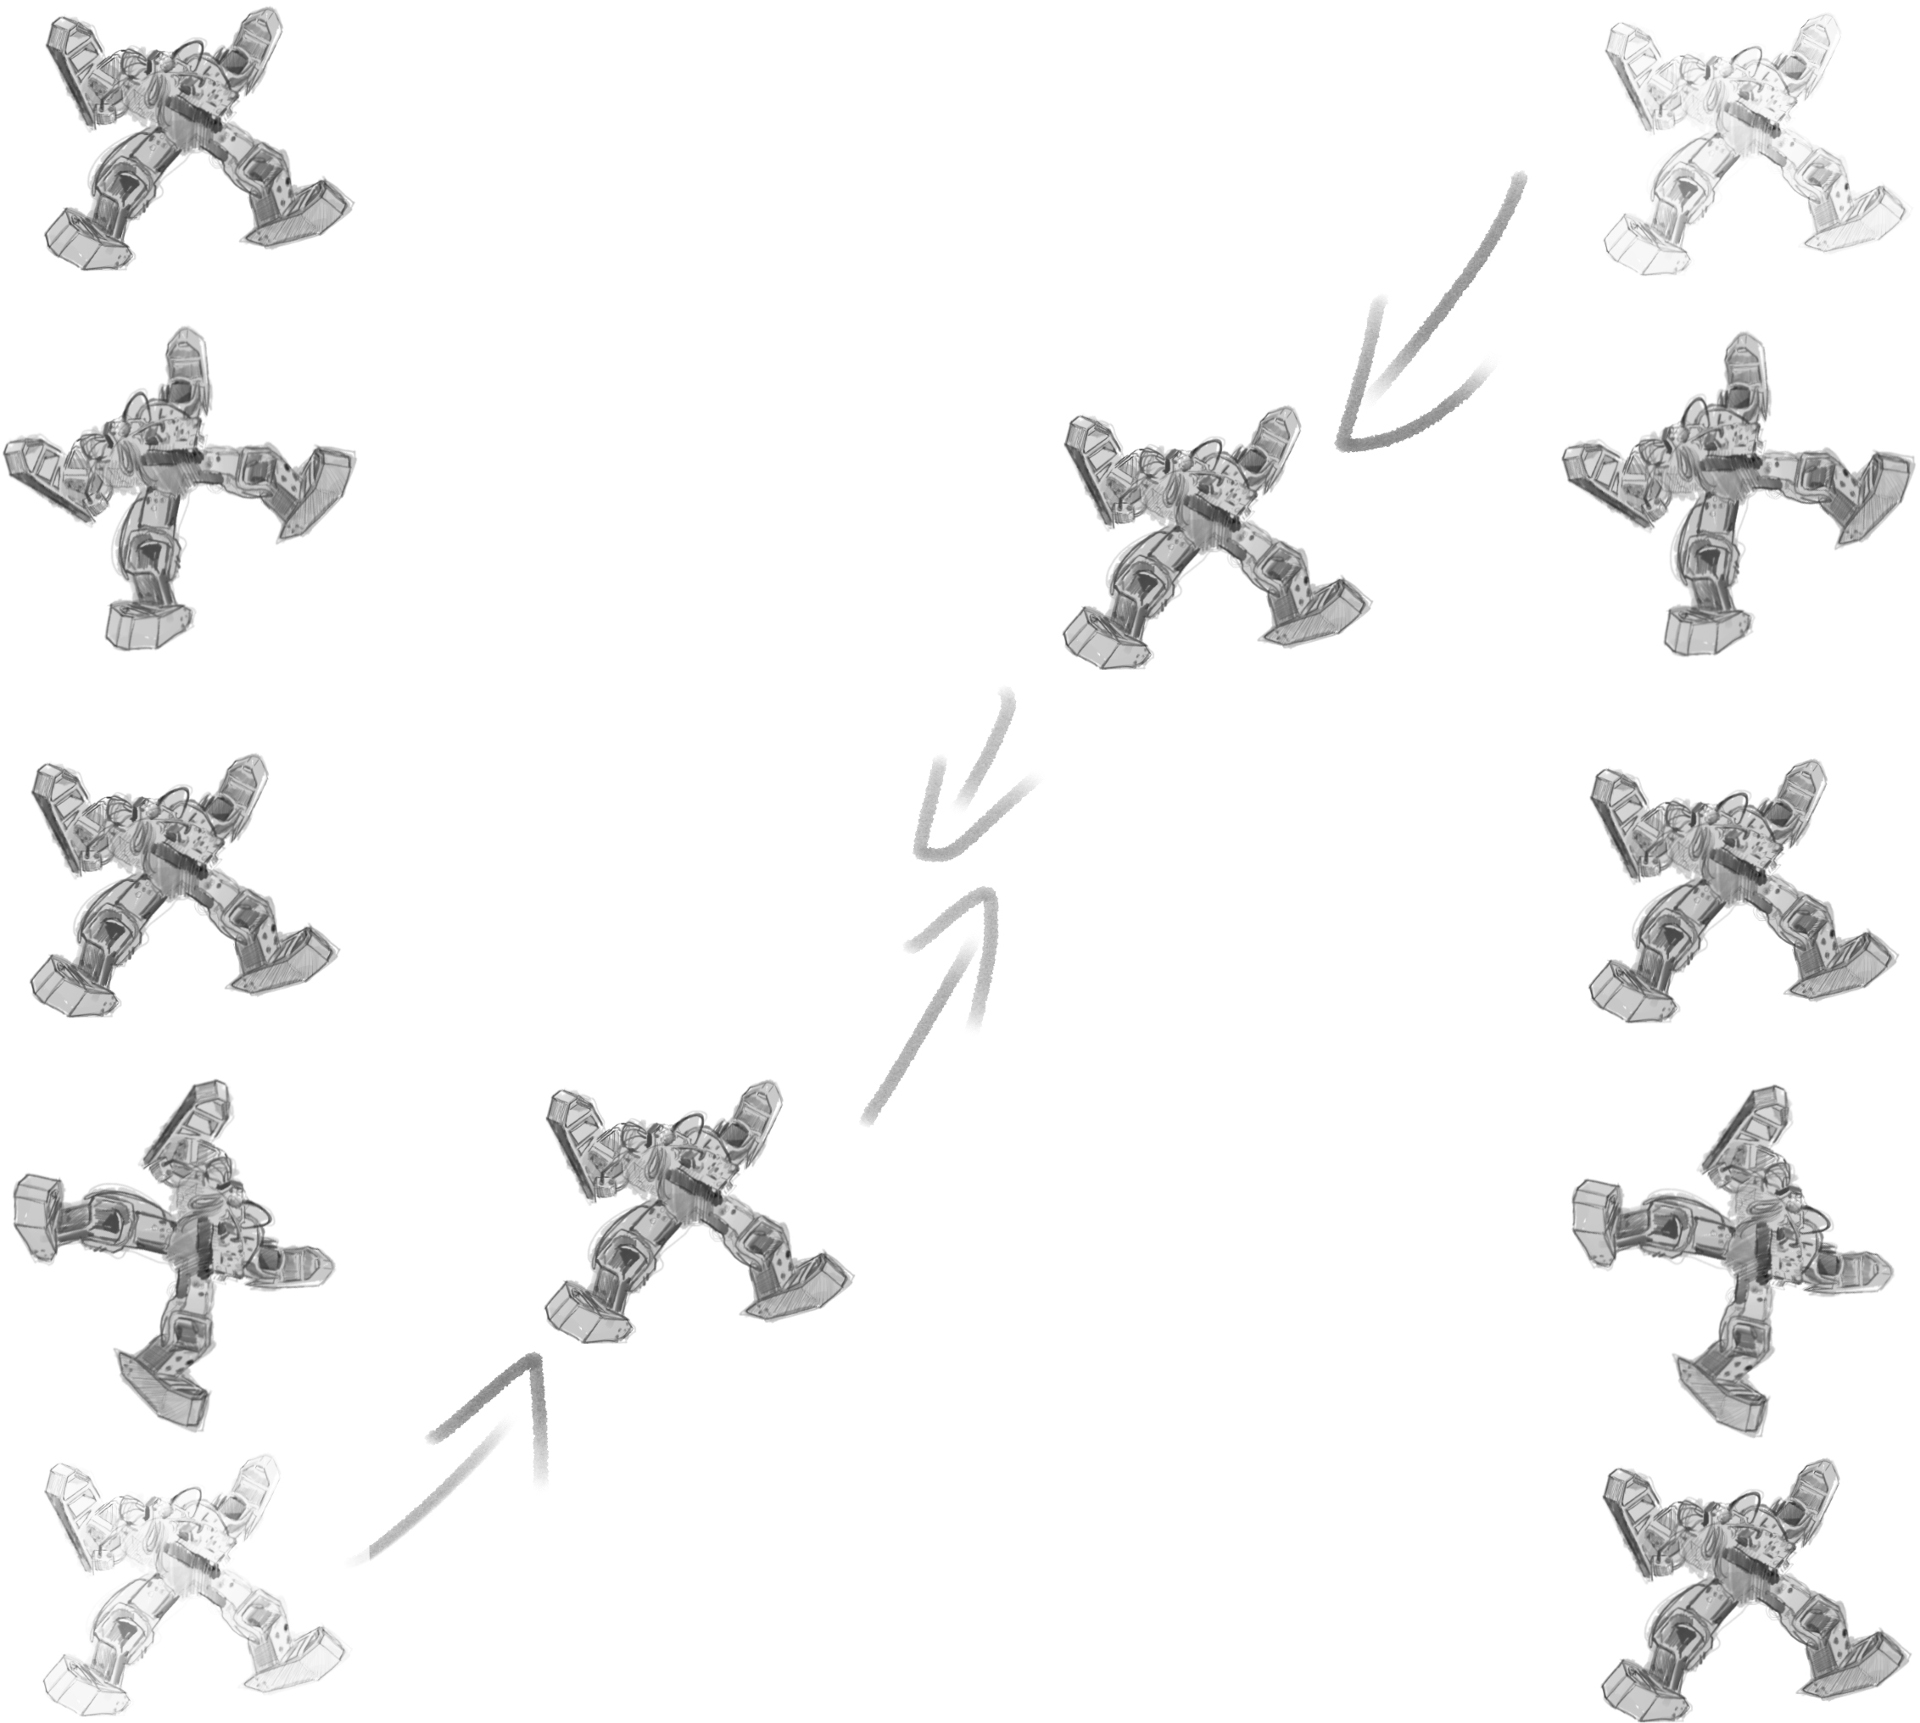
\includegraphics[scale=0.5]{reveildessin}
\caption{Dessin original des étudiants d'art de Bilbao}
\label{chore}
\end{figure}


\begin{figure} [H]
\centering
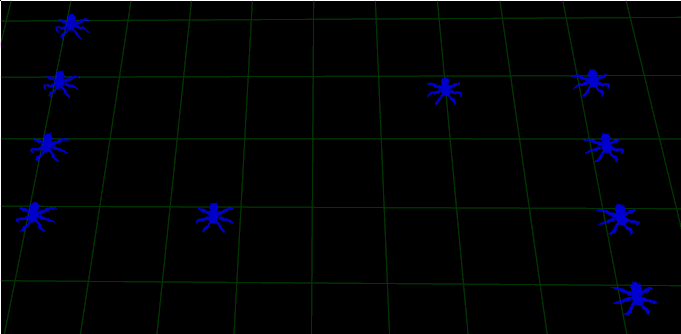
\includegraphics[scale=0.8]{reveil2}
\caption{Simulation du tableau avec notre interface simulationRainOfMusic}
\label{reveil}
\end{figure}

Une partie que nous avions commencé à travailler ensemble concernait un des derniers tableaux de la chorégraphie : la ronde que les robots font tout en s'arrêtant quelque fois pour tourner sur eux-mêmes. Pour cela, il fallait définir deux vitesses angulaires et un vecteur de déplacement pour que le robot puisse tourner en cercle et sur lui-même. La réalisation de ce mouvement s'est faite avec i-score et notre interface permettait de vérifier rapidement le résultat. 

Les artistes semblaient être intéressés par la visualisation que nous proposions. Par ailleurs, cette session de travail avec eux nous a permis de tester à nouveau notre logiciel, de régler certains bugs liés à des fonctionnalités récentes et donc d'améliorer notre travail. 

Ce fut donc une session nécessaire pour le développement et l'évaluation de notre logiciel. Un aspect qui n'a pas pu être abordé et qui aurait été intéressant pour la suite du projet : lancer une chorégraphie avec i-score, et vérifier les différences entre la réalité, les véritables mouvements des robots qui exécutent les commandes d'i-score, et la simulation, la chorégraphie réalisée dans la scène virtuelle de notre logiciel.

\subsection{Gestion du projet: calendrier et difficultés}

Dans cette partie, nous verrons la gestion du projet par rapport au calendrier que nous nous étions fixé. Puis nous verrons les difficultés que nous avons rencontrées. Un calendrier bilan est représenté sur la figure suivante \ref{cal}:

\begin{figure}[H]
  \begin{center}
  	\includegraphics[scale=0.7]{imgs/calendrierbis.png}
  	\caption{Calendrier bilan. En noir ce qui était prévu. En rouge ce qui était prévu mais qui n'a pas été fait. En vert ce qui a été fait mais qui n'était pas prévu}
  	\label{cal}
  \end{center}
\end{figure}

On remarque que finalement le calendrier de départ a subi beaucoup de changements. D'une part, la partie de simulation des mouvements des drones a été abandonnée car le projet s'est focalisé sur la mise en place des metabots en premier. D'autre part, la partie communication ne s'est pas déroulée comme prévu. L'intégration de la communication avec i-score dans simulationRainOfMusic (intégration de l'API d'OSSIA dans simulationRainOfMusic) nous a pris du temps. Une fois l'API en place, la communication avec i-score s'est établie assez facilement. 

Ensuite, l'ajout des panels dans l'interface de simulationRainOfMusic et la possibilité de modifier les paramètres des robots via ces panels a posé deux problèmes: la communication entre l'interface et le reste du logiciel, qui a donné lieu à la classe \verb|Parameter| et la synchronisation entre l'interface de simulationRainOfMusic et i-score. En effet, pour ce dernier, une boucle infinie peut facilement apparaître comme vu précédemment car les listener vers i-score et vers l'interface de simulationRainOfMusic déclenchent automatiquement la mise à jour des valeurs qu'ils écoutent. 

